\ttlfig{fig:fit}{Model Fit Measures}{
    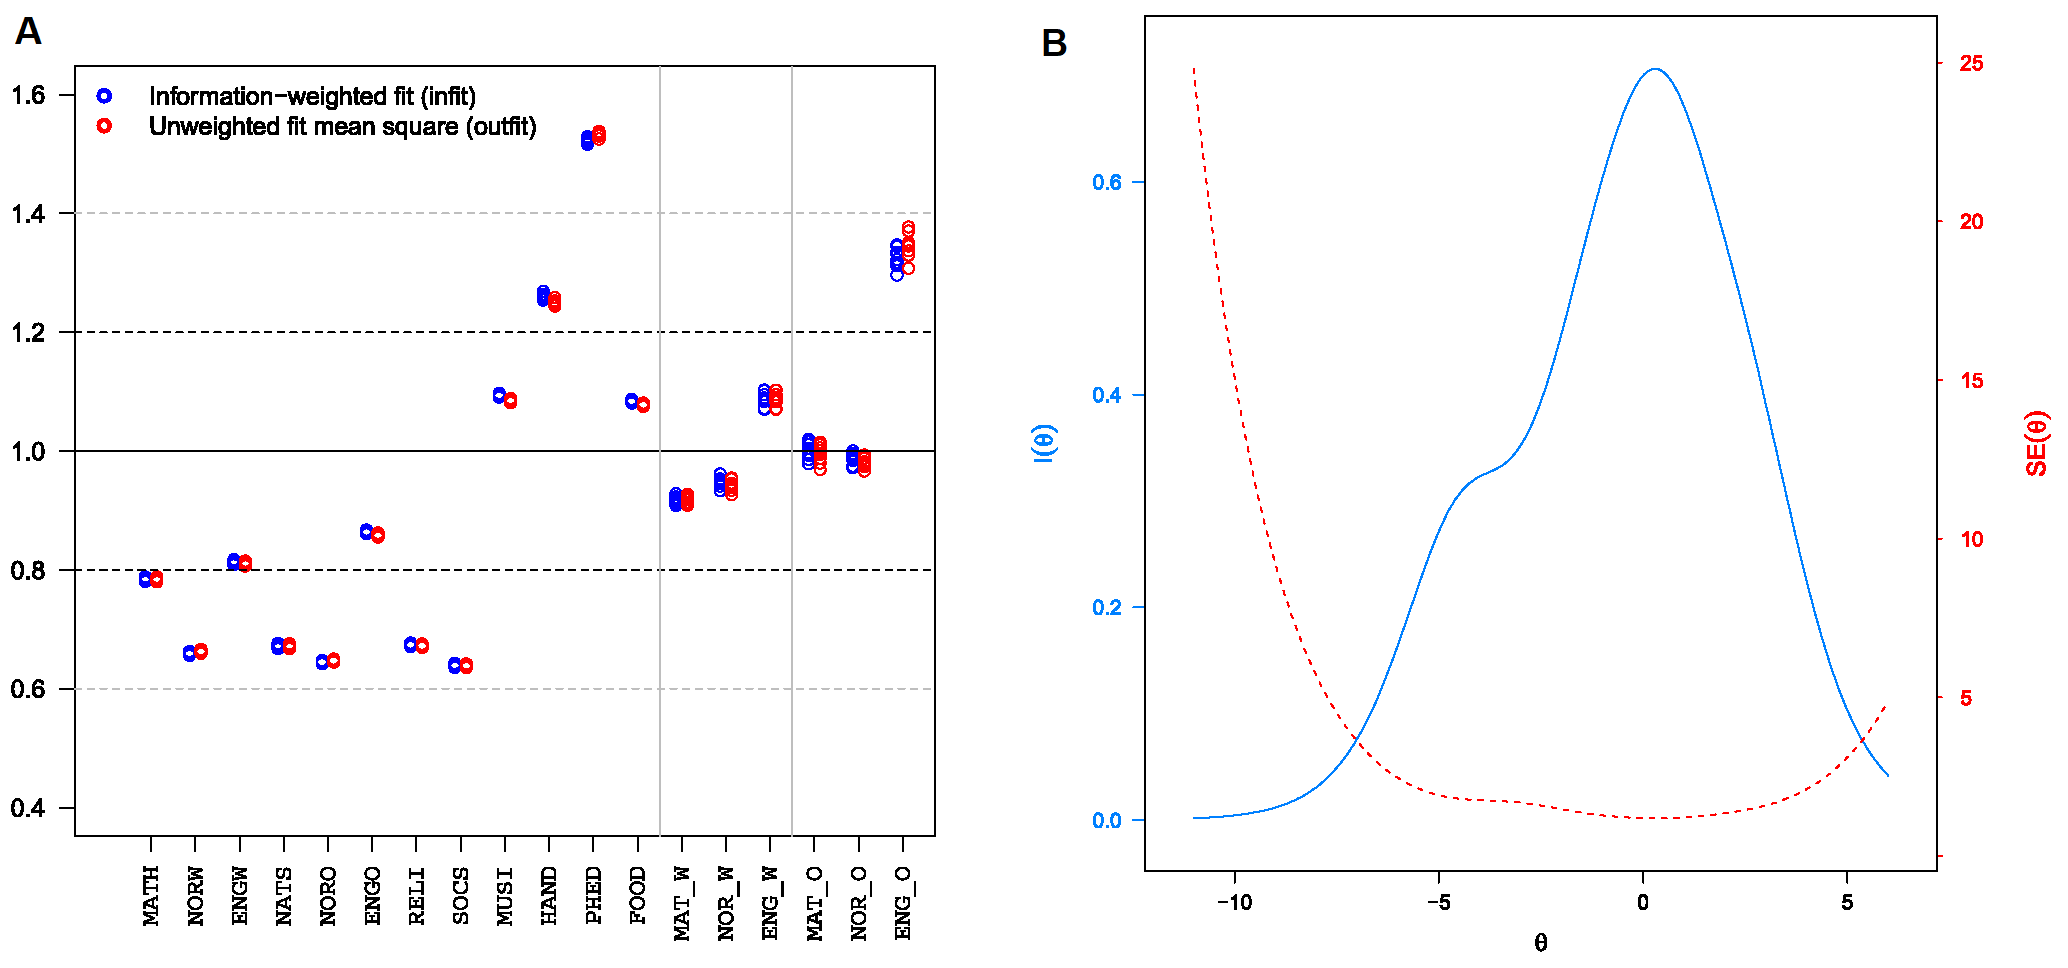
\includegraphics[width=1.5\textwidth]{./Figures/model_fit.png}
}{Panel A summarises model fit indices. A perfectly fit item in a Rasch model corresponds to infit and outfit statistics of $1$. Fit measure below $1$ indicate overfit where the item is more discriminating than the average item discrimination. Overfitting is usually not a problem comparing with underfitting. Empirical rules suggests close examination of items with infit and outfit statistics between $1.2$ and $1.5$ \parencite{wu:2016}. Panel B shows the information (blue, left scale) and standard error (red, right scale) curves of mathematics, suggesting good Rasch property over middle- to high-end of the competency scale.}
